\documentclass[10pt]{article}
\usepackage{llncsdoc}
\usepackage{hyperref}
\usepackage{graphicx}
\usepackage{array}
\usepackage{float}
\usepackage{fancyvrb}
\usepackage{amsmath}
\usepackage{multicol}
\usepackage{mathtools}
\usepackage{algpseudocode}
\usepackage{varwidth}
\DefineVerbatimEnvironment{code}{Verbatim}{fontsize=\small}
\DefineVerbatimEnvironment{example}{Verbatim}{fontsize=\small}


\begin{document}
\title{Improvements/Modifications to the algorithm for MAUT based critiquing}
\author{Bharath Reddy}
\maketitle

\tableofcontents

\pagebreak
\section{MAUT described in \cite{zhang}}
%probably write the missing functions here, calc utility and value() function.


\begin{figure}
    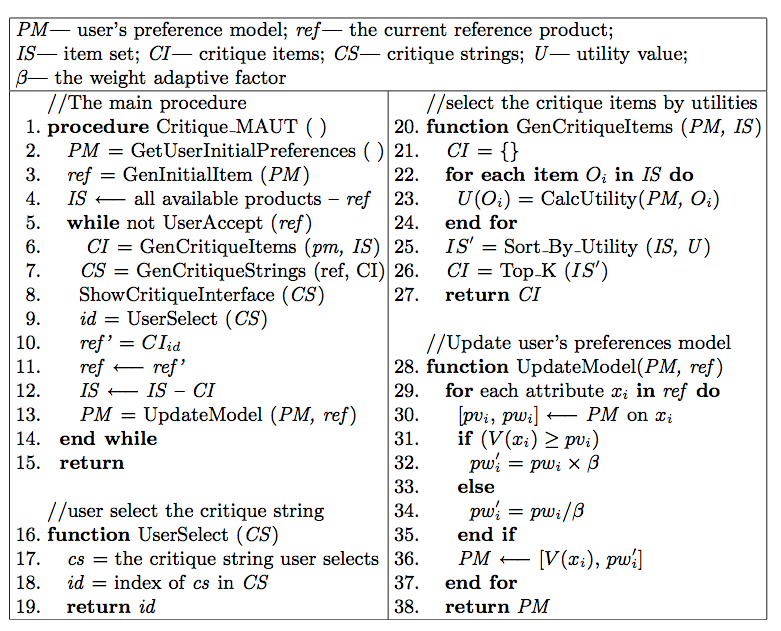
\includegraphics[width=1.0\textwidth]{paperAlgo.png}
  \caption{Algorithm described in the paper. Reference: \cite{zhang}}
  \centering
\label{fig:paperAlgo}
\end{figure}

In addition to the functions defined above, $CalcUtility(PM, u)$ is defined as follows:\\
def CalcUtility(PM, u):\\
\\
\noindent\fbox{%
\begin{varwidth}{\dimexpr\linewidth-2\fboxsep-2\fboxrule\relax}
\begin{algorithmic}[1]
\State $retVal = 0$
\For{i = 1 to numAttributes}
	\State $retVal += weight(attr[i])*value(attrValue(u, i), attr[i])$
\EndFor
\State return retVal
\end{algorithmic}
\end{varwidth}%
}
\\
\\
\\
\textbf{Updating value functions of nominal attributes:}\\
In each cycle, value functions of nominal attributes are updated instead of their weights.
Let $v_1, v_2, v_3,\hdots v_k$ be $k$ possible values of a nominal attribute $N$(say manufacturer).
Value associated with each of $v_1, v_2, v_3,\hdots, v_k$ is initialized to $1/k$ at the beginning of interaction.
In the first cycle, if selected product's manufacturer is $v_1$, value associated with $v_1$ is changed to $(1+\gamma)/(k+\gamma)$; and the value associated with $v_2, v_3, \hdots, v_k$ will be $1/(1+\gamma)$ in the next cycle.\\
In general, in cycle $t$,  each of $v_1, v_2, v_3,\hdots, v_k$ is multiplied by $(1 + t\gamma)$; if $v_p$ is the value of attribute $N$ in the selected product, then value associated with $v_p$ is increased by $\gamma$ and all the value functions associated with attribute $N$ are then normalized (so they all sum up to 1)  by dividing them all by $(1+ (t+1)\gamma)$\\
We get the least number of interaction cycles when $\gamma = 0.5$










\section{Modifications/Improvements done}
\subsection{Additive Model for updating attribute weights}
\label{sec:first}
\textbf{function} UpdateModel(PM, ref) is modified as follows:\\
\\
def UpdateModel(PM, ref):\\
\noindent\fbox{%
\begin{varwidth}
{\dimexpr\linewidth-2\fboxsep-2\fboxrule\relax}
\begin{algorithmic}
\If {$V(x_i)\geq pv_i$}
    $pw_i' = pw_i + \beta$
\EndIf
    \State $PM\gets [V(x_i),pw_i']$
\end{algorithmic}
\end{varwidth}
}
\\
\\
We increase the weight of attributes that need to have more weight in the next cycle. The weight of other attributes automatically decreases (compared to their previous weights) when normalization is done.
$\beta$ = 0.5 gives the best results in offline evaluations and in-fact performs better than the 
algorithm in Figure ~\ref{fig:paperAlgo}. Results are shown in Table ~\ref{tab:results}

%\State $R \gets BoundedGreedySelection $




\subsection{Diverse Critiques in every cycle}
A variant of \textit{\textbf{Bounded Greedy Selection}} algorithm described in \cite{mcginty} was used to generate diverse critiques in every cycle.
The function \textit{GenCritiqueItems(PM, IS)} is modified as follows:\\
\\
def GenCritiqueItems(PM, IS):\\
\noindent\fbox{%
\begin{varwidth}{\dimexpr\linewidth-2\fboxsep-2\fboxrule\relax}
\begin{algorithmic}[1]
\State R = \{\}
\State CB' = IS
\For{i = 1 to k}
	\State sort CB' by Quality(i, R, PM) for each case in IS
	\State R = R + First(CB')
	\State CB' = CB' - First(CB')
\EndFor
\State return R
\end{algorithmic}
\end{varwidth}%
}
\\
\\
def Quality(i, R, PM):\\
\noindent\fbox{%
\begin{varwidth}{\dimexpr\linewidth-2\fboxsep-2\fboxrule\relax}

\begin{algorithmic}[1]
\If{R == \{\}} return 0;
\Else
\State $retVal = \alpha \times utility(i, PM)$
\State $disSim = \sum_{r_j \in R} (1-critiqueSim(i,r_j))/|R|$
\State $retVal += (1-\alpha) \times disSim$
\State return retVal
\EndIf
\end{algorithmic}
\end{varwidth}%
}
\\
\\
$critiqueSim(a, b)$ returns the extent of overlap between the individual attribute directions of products $a$ and $b$.
We get the best results when $\alpha = 0.5$.
Introducing diverse critiques in every cycle results in significant improvement in the number of interaction cycles (Table ~\ref{tab:results}) and it also improves user experience (Users don't prefer critiques being very similar to each other).





\subsection{Selectively Updating value functions of nominal attribute values}
In the implementation of MAUT algorithm described in \cite{zhang}, $\gamma$ for updating value function of nominal attributes is fixed at 0.5 in each cycle.
If $k$ is the value of the attribute N selected in a cycle and $R$ is the list of values of attribute $N$ of the top-K products other than the selected products, we define
\begin{equation}
\gamma = \frac{\#\: of\: alternatives\: to\: k\: in\: R}{|R|}
\end{equation}
If attribute $N$ = "Manufacturer"; $\gamma$ = 1 when manufacturer of all the remaining products is different from the selected product's manufacturer and also different from each other.
$\gamma$ = 0 when manufacturer of all remaining products is same as the selected product's manufacturer.
This is similar to weighted MLT described in \cite{wmlt}.
Varying the value of $\gamma$ according to the other products' attribute values results in a significant improvement in the number of interaction cycles.

\subsection{Additional Preference to products satisfying the most recent user selected critique string}
If user selects the critique string "Lower Price, Higher Resolution but Higher Weight", we give an additional importance to the products that satisfy the critique string. 
Modified $CalcUtility$ function is as follows:\\
\\
def CalcUtility(PM, u):\\
\noindent\fbox{%
\begin{varwidth}{\dimexpr\linewidth-2\fboxsep-2\fboxrule\relax}
\begin{algorithmic}[1]
\State $retVal = 0$
\For{i = 1 to numAttributes}
	\State $retVal += weight(attr[i])*value(attrValue(u, i), attr[i])$
\EndFor
\State $retVal += critiqueOverlap(u, previousSelectedProduct)$
\State return retVal
\end{algorithmic}
\end{varwidth}%
}
\\
\\







\subsection{Similar Products in first cycle}
In the algorithm described in the paper, weights of all numeric attributes were initialized to $1/n$ and the top K utility products are the presented to the user in the first cycle. Hence, the top K products presented in the first cycle are the same irrespective of initial preferences given by the user. 
Instead of presenting top K utility products, we will present the most similar prducts to user's initial peferences in the first cycle. This modification leads to updating weights in the right direction such that the target product shows up quickly in list of top K products. This 


\subsection{Taking history of user selected products into account}
\label {sec:history}
In Line 29 of Figure ~\ref{fig:paperAlgo},  $ref$ is the product selected by user in the previous cycle.
Preference model is updated using only the most recently selected product's attribute values.
We can instead maintain a list of products selected by the user in previous cycles and update the model using a weighted average of these products' attributes.
The modified function $UpdateModel(PM, ref)$ is as follows:\\
\\
\textbf{def} UpdateModel(PM, refList):\\
\noindent\fbox{%
\begin{varwidth}{\dimexpr\linewidth-2\fboxsep-2\fboxrule\relax}
\begin{algorithmic}[1]
\For{each attribute $x_i$}
	\State $ref[x_i] = \sum_{p \in refList} hw_i \times p[x_i]/(\sum_i hw_i)$

\EndFor
\For{each attribute $x_i$ in ref}
	\State $\hdots$
	\State /*multiplicative or additive model used for updating weights*/
	\State $\hdots$
\EndFor


\end{algorithmic}
\end{varwidth}%
}
\\
\\


\subsection{Introducing Diversity as a function of how preference model changes}
We define a certain threshold (around 5 \% of (maxV-minV)) for each of the numeric attributes. If the difference in the attribute values of the reference product and selected product is within the threshold, the weight of that attribute is not updated and is included in the set $N$. The value of $\alpha$ in Quality(i, R, PM) is defined as:
\begin{equation}
\alpha = \frac{|N|}{|R|}
\end{equation}

$\alpha$ = 1 when values of all the numeric attributes fall within the defined threshold of the reference product. In this case we assume that the preference model is stable, and the topK utility products are returned.
$\alpha$ = 0 when values of all numeric attributes are out of threshold. In this case, we assume that the user isn't very sure of his current preferences and thus products with very diverse critiques are returned.

\subsection{Selectively updating weights of numeric attributes}
\label{sec:last}
Consider the case when in a particular cycle, all the products(cameras) displayed to the user have a "Lower Resolution". In that case user is forced to choose a camera with "Lower Resolution". The algorithm in \cite{zhang} would reduce the weight of attribute "Resolution" by a factor of 2. We should not actually increase/decrease the weight of attribute "Resolution" because we can't infer user's preference on the attribute "Resolution".\\
Consider another case when 4 out of 5displayed products have a "Lower Resolution" compared to the reference product and only one product out of the 5 has a "Higher Resolution". If user selects the product that has a higher resolution,we should increase the weight of "Resolution" attribute by a factor greater than just 2, since we see that user has rejected 4 cameras that have lower resolution and thus has a strong preference for the attribute "Resolution".\\

The factors with which weights of an MIB attribute are updated are shown in Table ~\ref{tab:selective}. The factors for LIB attribute will also be similar.


\begin{table}
\centering
    \caption{Factor with which weights are multiplied for an \textbf{MIB} attribute in line 32 in Figure ~\ref{fig:paperAlgo}}
\label{tab:selective}
    \begin{tabular}
{ >{\textbf} m{2.2cm} >{\centering\arraybackslash} m{3.0cm} >{\centering\arraybackslash} m{2.8cm} >{\centering\arraybackslash} m{2.7cm}  }
    \hline
    \hline
	Number of critiques with "low" resolution                      & Number of critiques with "high" resolution   
	& Critique with "low" resolution selected   			& Critique with "high" resolution selected\\
    \hline

5	&0	&1		&1\\
4	&1	&1/2 	&4\\
3 	&2	&1/2 	&3\\
2 	&3	&1/3	&2\\
1 	&4	&1/4	&2\\
0	&5	&1		&1\\


\hline
\hline
\end{tabular}
\end{table}





\section{Results}
Following are the results obtained for offline evaluation experiments done on Camera data set.
The Camera data set has 171 cases. The original Camera data set at \url{http://josquin.cs.depaul.edu/~rburke/research/downloads/camera.zip} had 210 cases. 39 cases with missing values have been removed. Results for all the modifications from Sec ~\ref{sec:first} to Sec ~\ref{sec:last}  have been tabulated in Table ~\ref{tab:results} and the plot of the results is shown in Figure ~\ref{fig:results}.
All the experiments have been performed using the same query set of 1710 queries.
\label{sec:results}

%---------------------------------------------------------
\begin{table}
\centering
    \caption{Average Number of interaction cycles for q1, q3, q5}
\label{tab:results}
    \begin{tabular}{ >{\textbf} m{5cm} >{\centering\arraybackslash} m{1.3cm} >{\centering\arraybackslash} m{1.3cm} >{\centering\arraybackslash} m{1.3cm} >{\centering\arraybackslash} m{2.8cm} }
    \hline
    \hline
	Camera DataSet                      & q1   & q3   & q5   & \%improvement(wrt MAUT in \cite{zhang} and q1) \\
    \hline

MAUT as described in paper                                       & 9.21 & 4.08 & 2.01 &               \\
\hline
MAUT-additive model (2.1)                                        & 8.72 & 3.68 & 1.88 & 5.4           \\
\hline
Diverse critiques in every cycle (2.2)                           & 7.83 & 3.12 & 1.38 & 15            \\
\hline
Selectively updating value functions of nominal attributes (2.3) & 7.13 & 3.45 & 1.73 & 22.6          \\
\hline
Additional pref to products satisfying most recent critique(2.4) & 6.42 & 2.8  & 1.37 & 30.3          \\
\hline
Similar Products in First Cycle(2.5)                             & 6.23 & 2.04 & 1.22 & 32.4          \\
\hline
History of user selected Products (2.6)                          & 8.66 & 3.67 & 1.83 & 6             \\
\hline
Diversity as function of change in PM (2.7)                      & 7.62 & 3.04 & 1.33 & 17.3              \\
\hline
Selectively updating weights of numeric attributes(2.8)          & 9.62 & 4.42 & 2.11 & -4.4     \\         

 \hline
    \hline
    \end{tabular}

\end{table}

%---------------------------------------------------------

\begin{figure}
    \includegraphics[width=0.95\textwidth]{results.png}
  \caption{Number of interactions cycles for q1, q3, q5}
  \centering
\label{fig:results}
\end{figure}


\section{Further work}
\begin{itemize}

\item Utility of a product is currently estimated using a weighted sum of value functions of individual attributes.  additional terms that correspond to trade-offs between pairs of attributes can be introduced in utility function.

\item Inferring value functions of nominal attributes using the assumption of the market model - "No product is completely dominated by any other product".

\item UtilSim \cite{utilSim} learns user's preferences relatively quickly by exploiting the fact that user prefers one particular product over the other (K-1) products displayed to him. Algorithms to calculate utilties of products in each cycle can be used almost directly here


\item Evaluation has been done only in "Highly Focused Framework" where user selects the best/optimal product in each cycle and only one product is the target product. Evaluation has to be done in other scenarios like "Noise Based Framework" where sub-optimal choices will be selected, "Finding all Good items" when neighbors/dominators are also considered as targets etc.

\item Selectively updating weights of numeric attributes described in Section ~\ref{sec:last} has to be tried for additive model. With the update factors in Table ~\ref{tab:selective}, the performance is little worse compared to algorithm in \cite{zhang}. More experimentation has to be done to get the right update factors in Table ~\ref{tab:selective}

\item Methods other than the one mentioned in ~\ref{sec:history} need to be explored to exploit history better

\end{itemize}



\bibliography{llncs}
\bibliographystyle{plain}

\end{document}
